\chapter[Supporting Information for ``Paleomagnetism of the southwest Laurentia large igneous province and Cardenas Basalt: pulsed magmatism during rapid late Mesoproterozoic plate motion"][Supporting Information--SWLLIP]{Supporting Information for ``Paleomagnetism of the southwest Laurentia large igneous province and Cardenas Basalt: pulsed magmatism during rapid late Mesoproterozoic plate motion"}

\begin{figure}
\centering
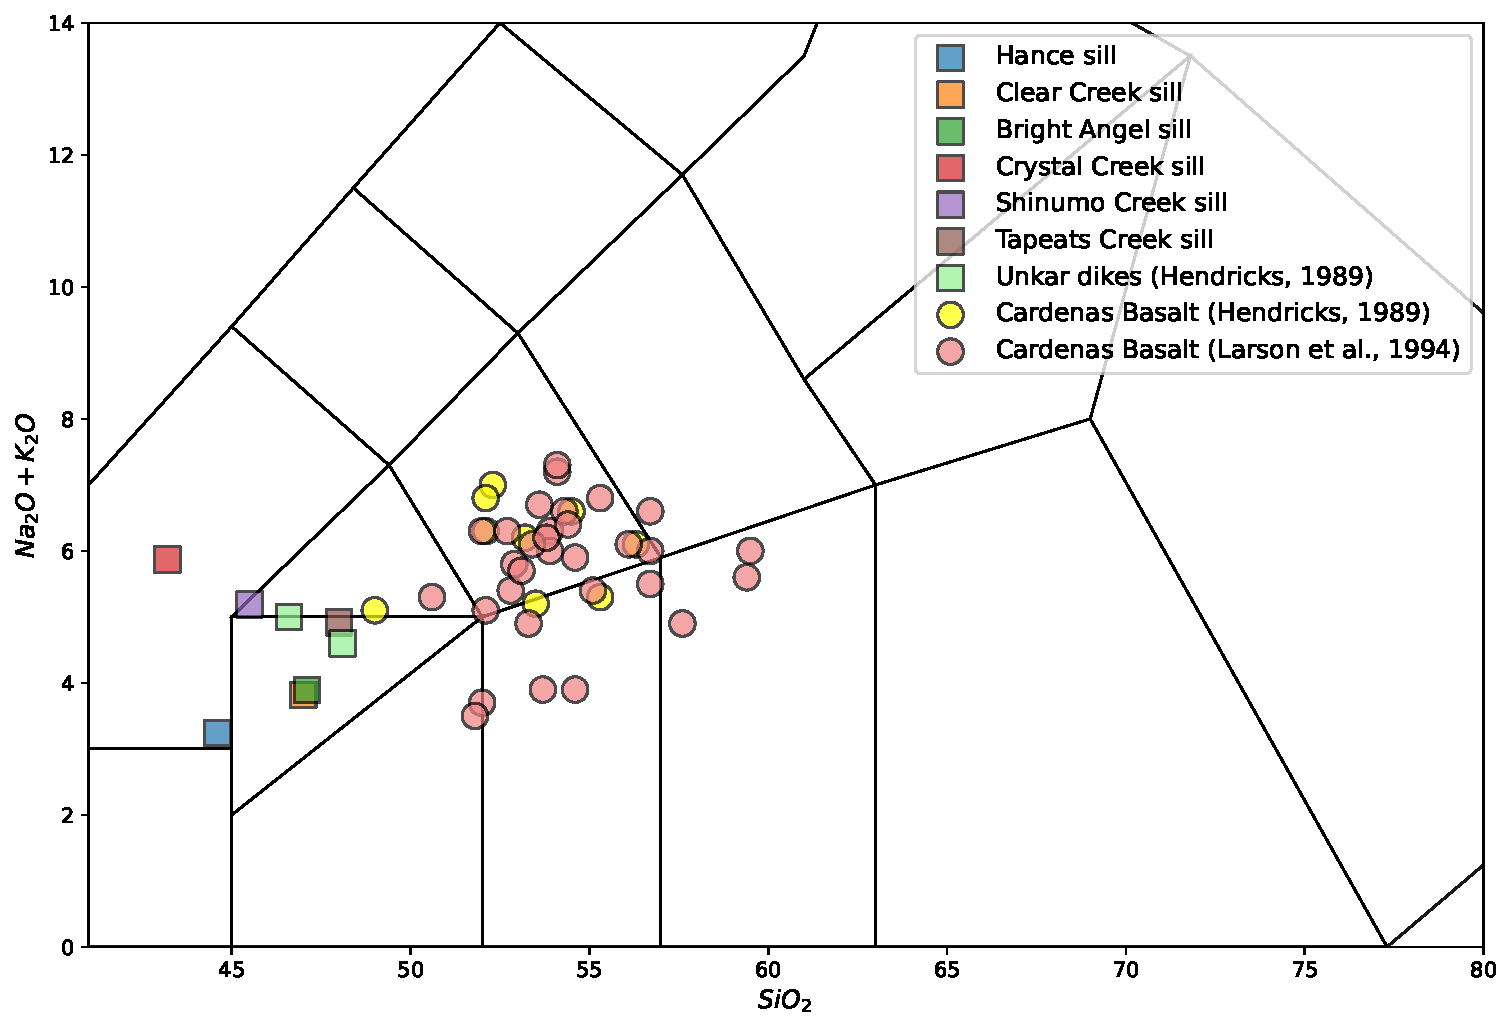
\includegraphics[width=\textwidth]{figure/Zhang2024b/Cardenas_Unkar_geochem_major.pdf}
\caption[Major element geochemical data of the Cardenas Basalt and diabase intrusions in the Unkar Group.]{Total alkali-silica diagram of the Cardenas Basalt and mafic intrusions within the Unkar Group. The sills and dikes typically have lower silica content (basalt) than the Cardenas Basalt (basaltic trachy-andesite). Data for the Cardenas Basalt are from \cite{Hendricks1989a} and \cite{Larson1994a}. Data for the intrusions are from \cite{Hendricks1989a}.}
\label{fig:geochem_major}
\end{figure}

\begin{figure}
\noindent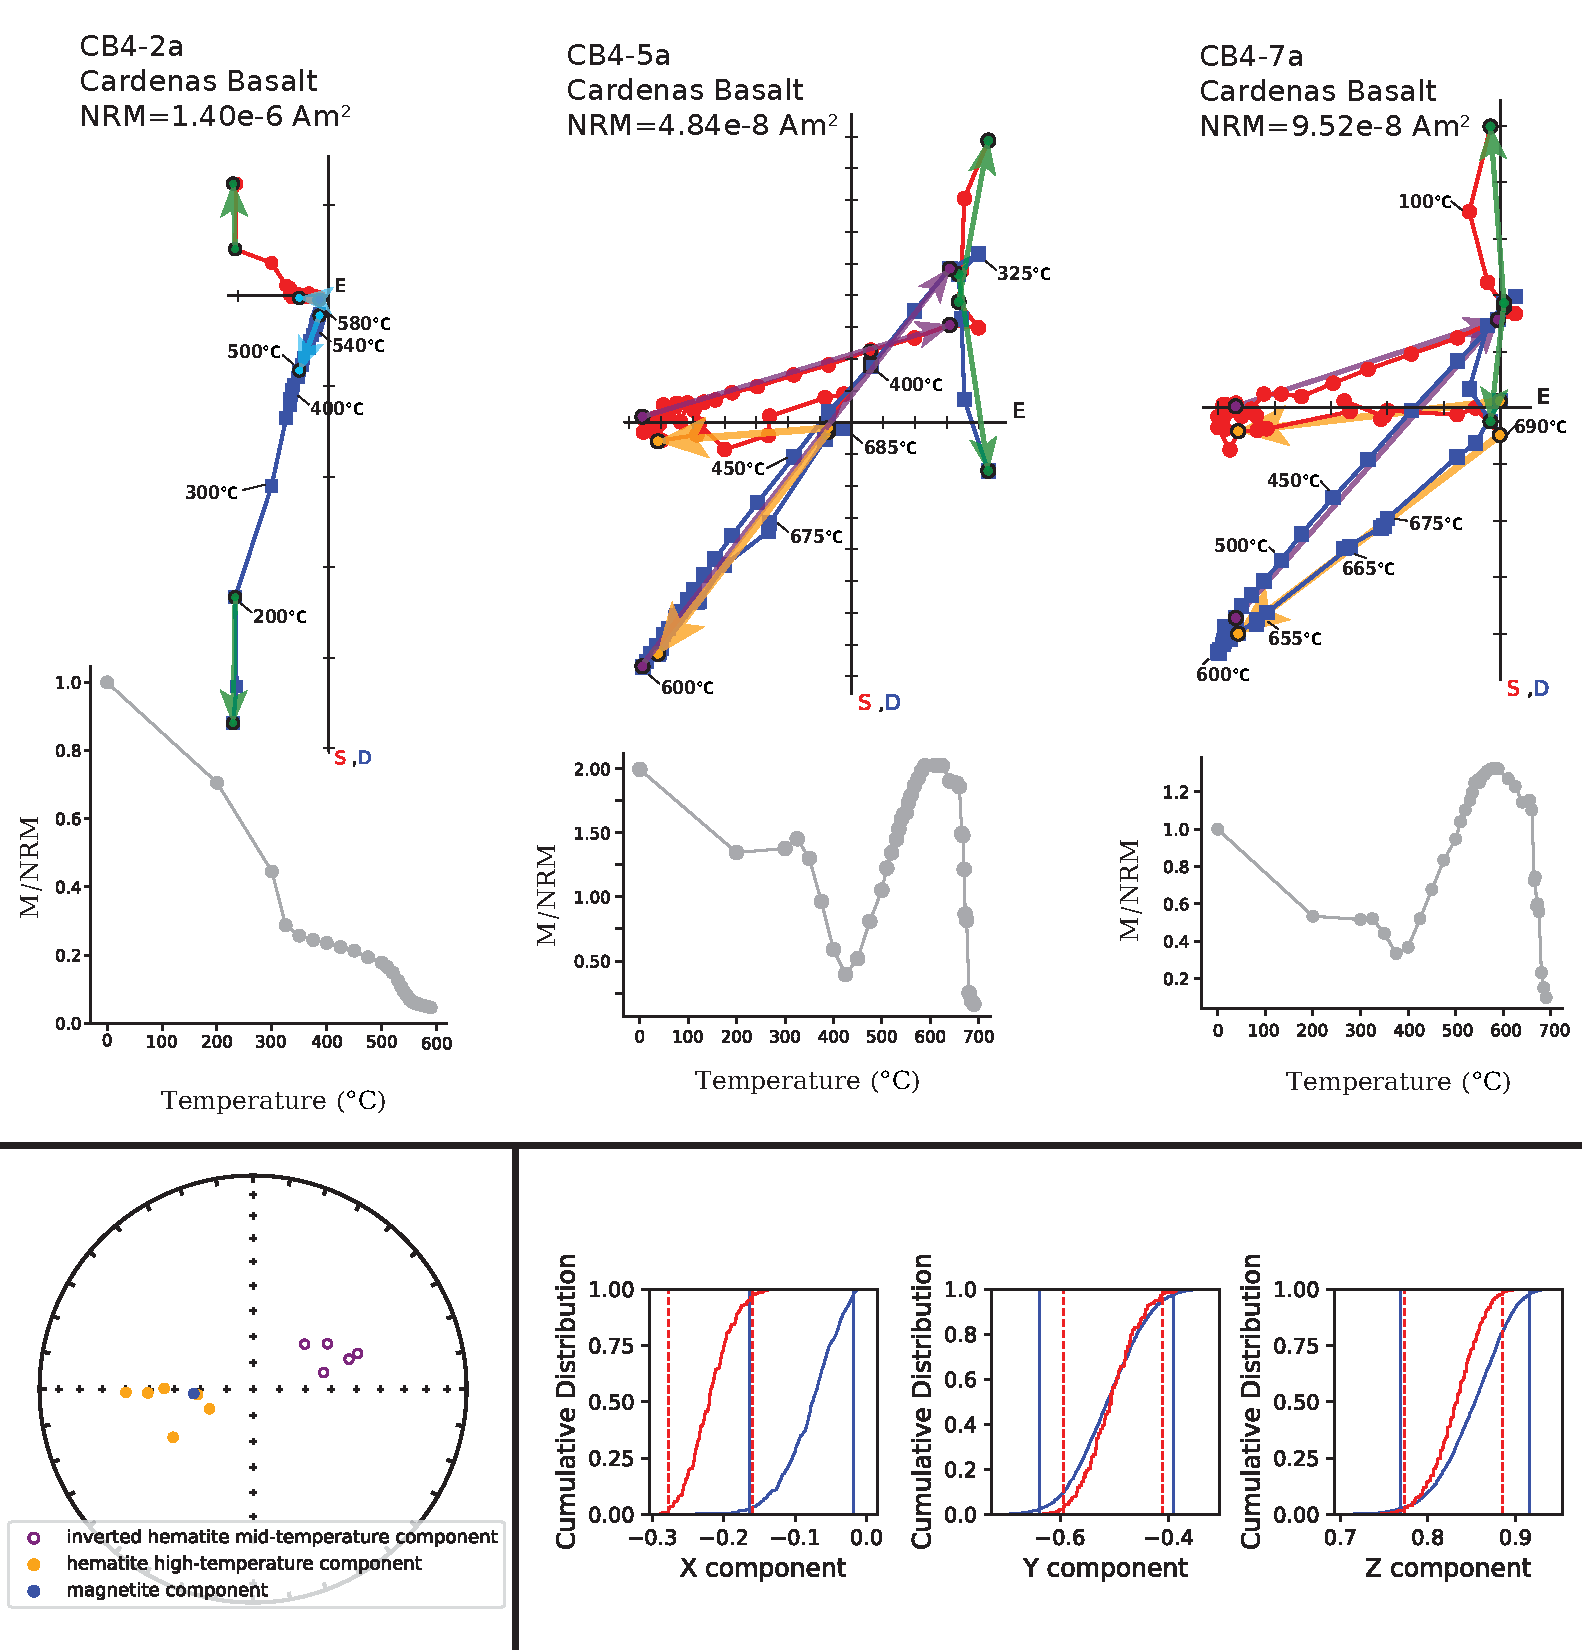
\includegraphics[width=5.8 in]{figure/Zhang2024b/SI_CB4.pdf}
\caption[Paleomagnetic data of Cardenas Basalt lava flow site CB4.]{\footnotesize Top panel: Thermal demagnetization data of paleomagnetic specimens collected near the bottom of lava flow CB4. Specimen CB4-2a has a demagnetization behavior similar to other lava flows--after the removal of the present day local field overprint, an origin-trending magnetite-carrying characteristic component unblocks up to 580\textdegree C. However, for all other specimens, after the removal of the present day local field overprint by $\sim$300\textdegree C (green vector), their total magnetic moments typically increase as the thermal demagnetization approaches $\sim$600\textdegree C. This mid-temperature component is followed by an origin-trending decay approaching the N\`eel temperature of hematite. Bottom panel: Bootstrap reversal test \citep{Tauxe1991a} of the mid-temperature and high-temperature remanence component of CB4. The directions pass the bootstrap reversal test and \cite{McFadden1990a} reversal test of  with a `C' classification. The high-temperature component that unblocks sharply near the hematite N\`eel temperature has the same polarity with titanomagnetite carried directions in other Cardenas Basalt flows. This similarity is consistent with the hematite forming from oxidation soon after eruption \citep{Haggerty1967a}. A likely origin of the antipodal component is that it is a self-reversed chemical remanent magnetization held by fine-grained hematite that formed as a result of inversion of maghemite precursors \citep{Hedley1968a, McClelland1987a, McClelland1993a, Swanson-Hysell2011a}. This self-reversal behavior is more likely than one that involves the reversal of the geomagnetic field after the emplacement of the CB4 lava flow. No reversed direction is observed in the adjacent lava flows and previous compilations of paleomagnetic data during this time suggest that the Cardenas lava flows were emplaced during a normal-polarity superchron \citep{Swanson-Hysell2019a, Driscoll2016b}.}
\label{fig:CB4_reversal_test}
\end{figure}

\begin{figure}
\noindent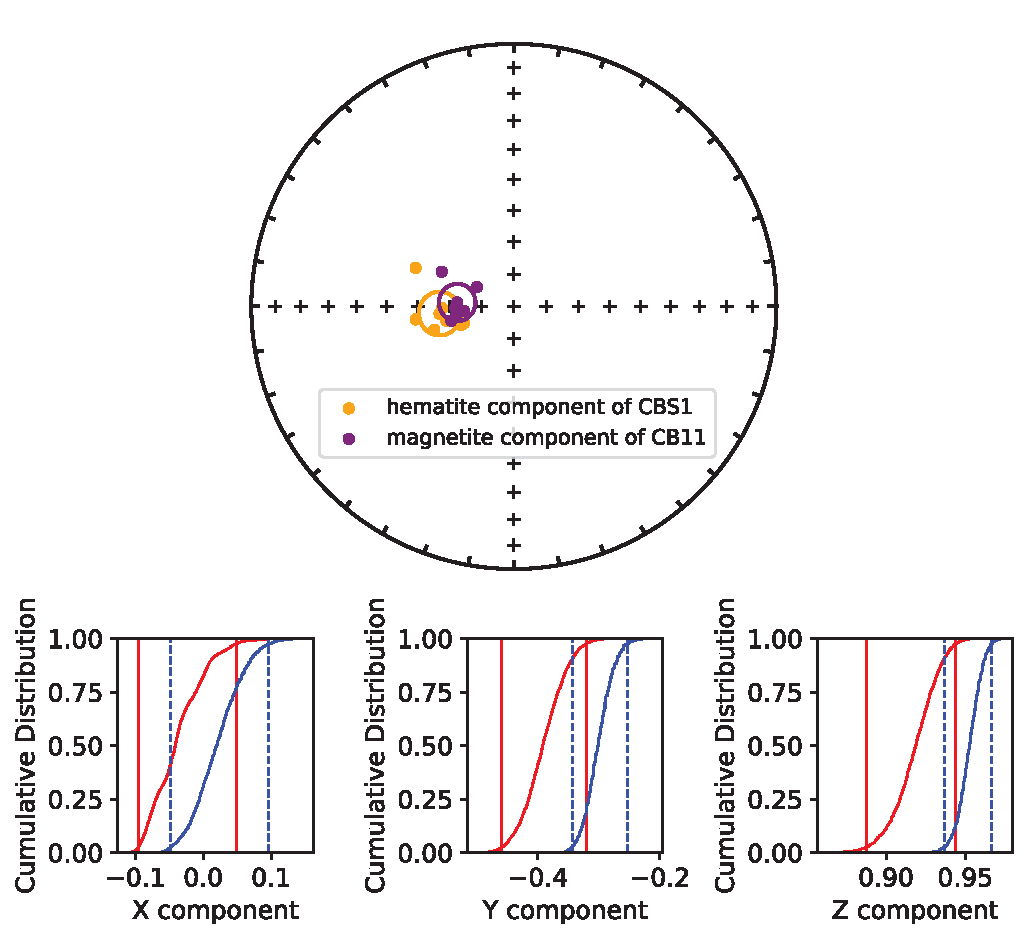
\includegraphics[width=5.8 in]{figure/Zhang2024b/SI_CBS1_CB11.pdf}
\caption[Paleomagnetic data of Cardenas Basalt lava flow site CB11 and the interflow sandstone site CBS1 below CB11.]{Top: Equal area plot showing the hematite magnetization specimen directions (orange) of the interflow sandstone CBS1 which is stratigraphically below the CB11 lava flow, whose magnetite magnetization directions are shown in purple. Bottom: Bootstrap common mean test of \cite{Tauxe1991a} between the specimens directions of the sandstone and the lava flow show a positive result. The specimen directions also passes a common mean test of \cite{McFadden1990a} with a `B' classification and have a positive support for sharing a common mean based on the Bayesian approach of \cite{Heslop2023a}.}
\label{fig:DV_tilt_test}
\end{figure}


\begin{figure}
\noindent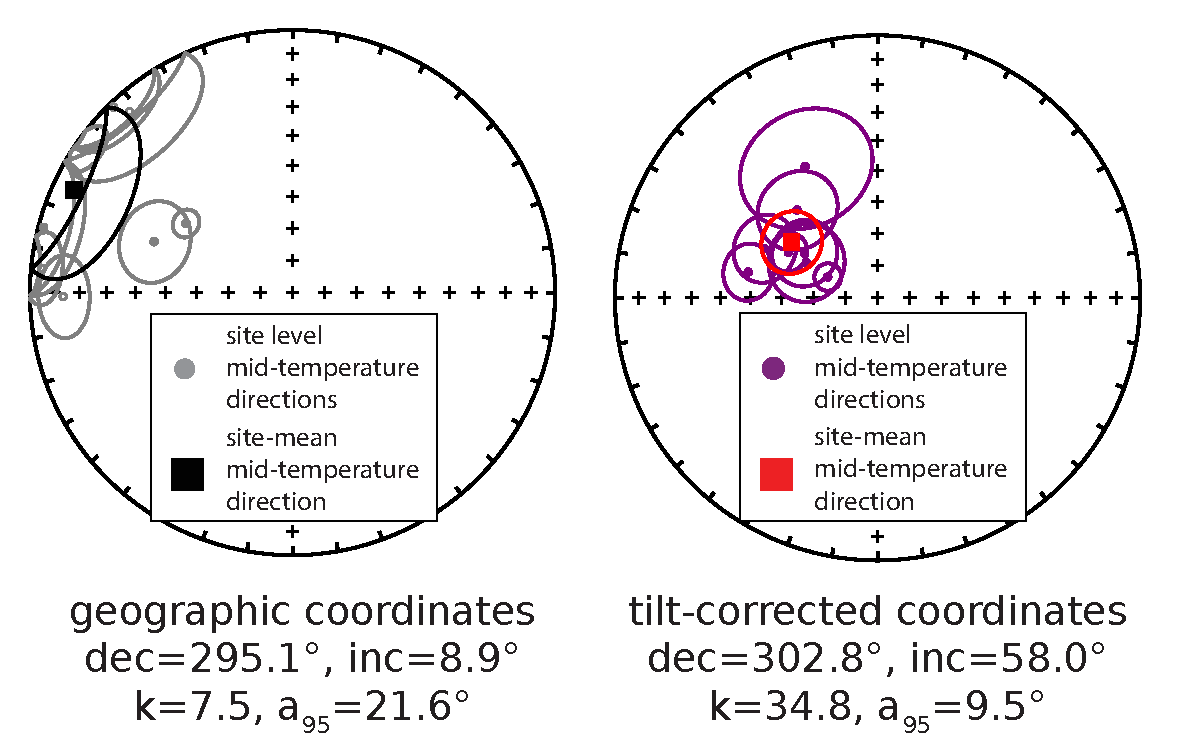
\includegraphics[width=5.8 in]{figure/Zhang2024b/SI_tilt_test.pdf}
\caption[Death Valley diabase sill paleomagnetic tilt test]{Equal area plots showing the site-level directions and site-mean directions of the Death Valley diabase sills that yielded coherent within-site thermal demagnetization results in both geographic coordinates (left) and tilt-corrected coordinates (right). The site-mean direction in geographic coordinates is dec=295.1\textdegree, inc=8.9\textdegree, n=8, k=7.5, a$_{95}$=21.6\textdegree. The site-mean direction in tilt-corrected coordinates is dec=302.8\textdegree, inc=58.0\textdegree, k=34.8, a$_{95}$=9.5\textdegree. Applying tilt correction to the sills significantly improves the grouping of the site level directions. }
\label{fig:DV_tilt_test}
\end{figure}

\begin{figure}
\noindent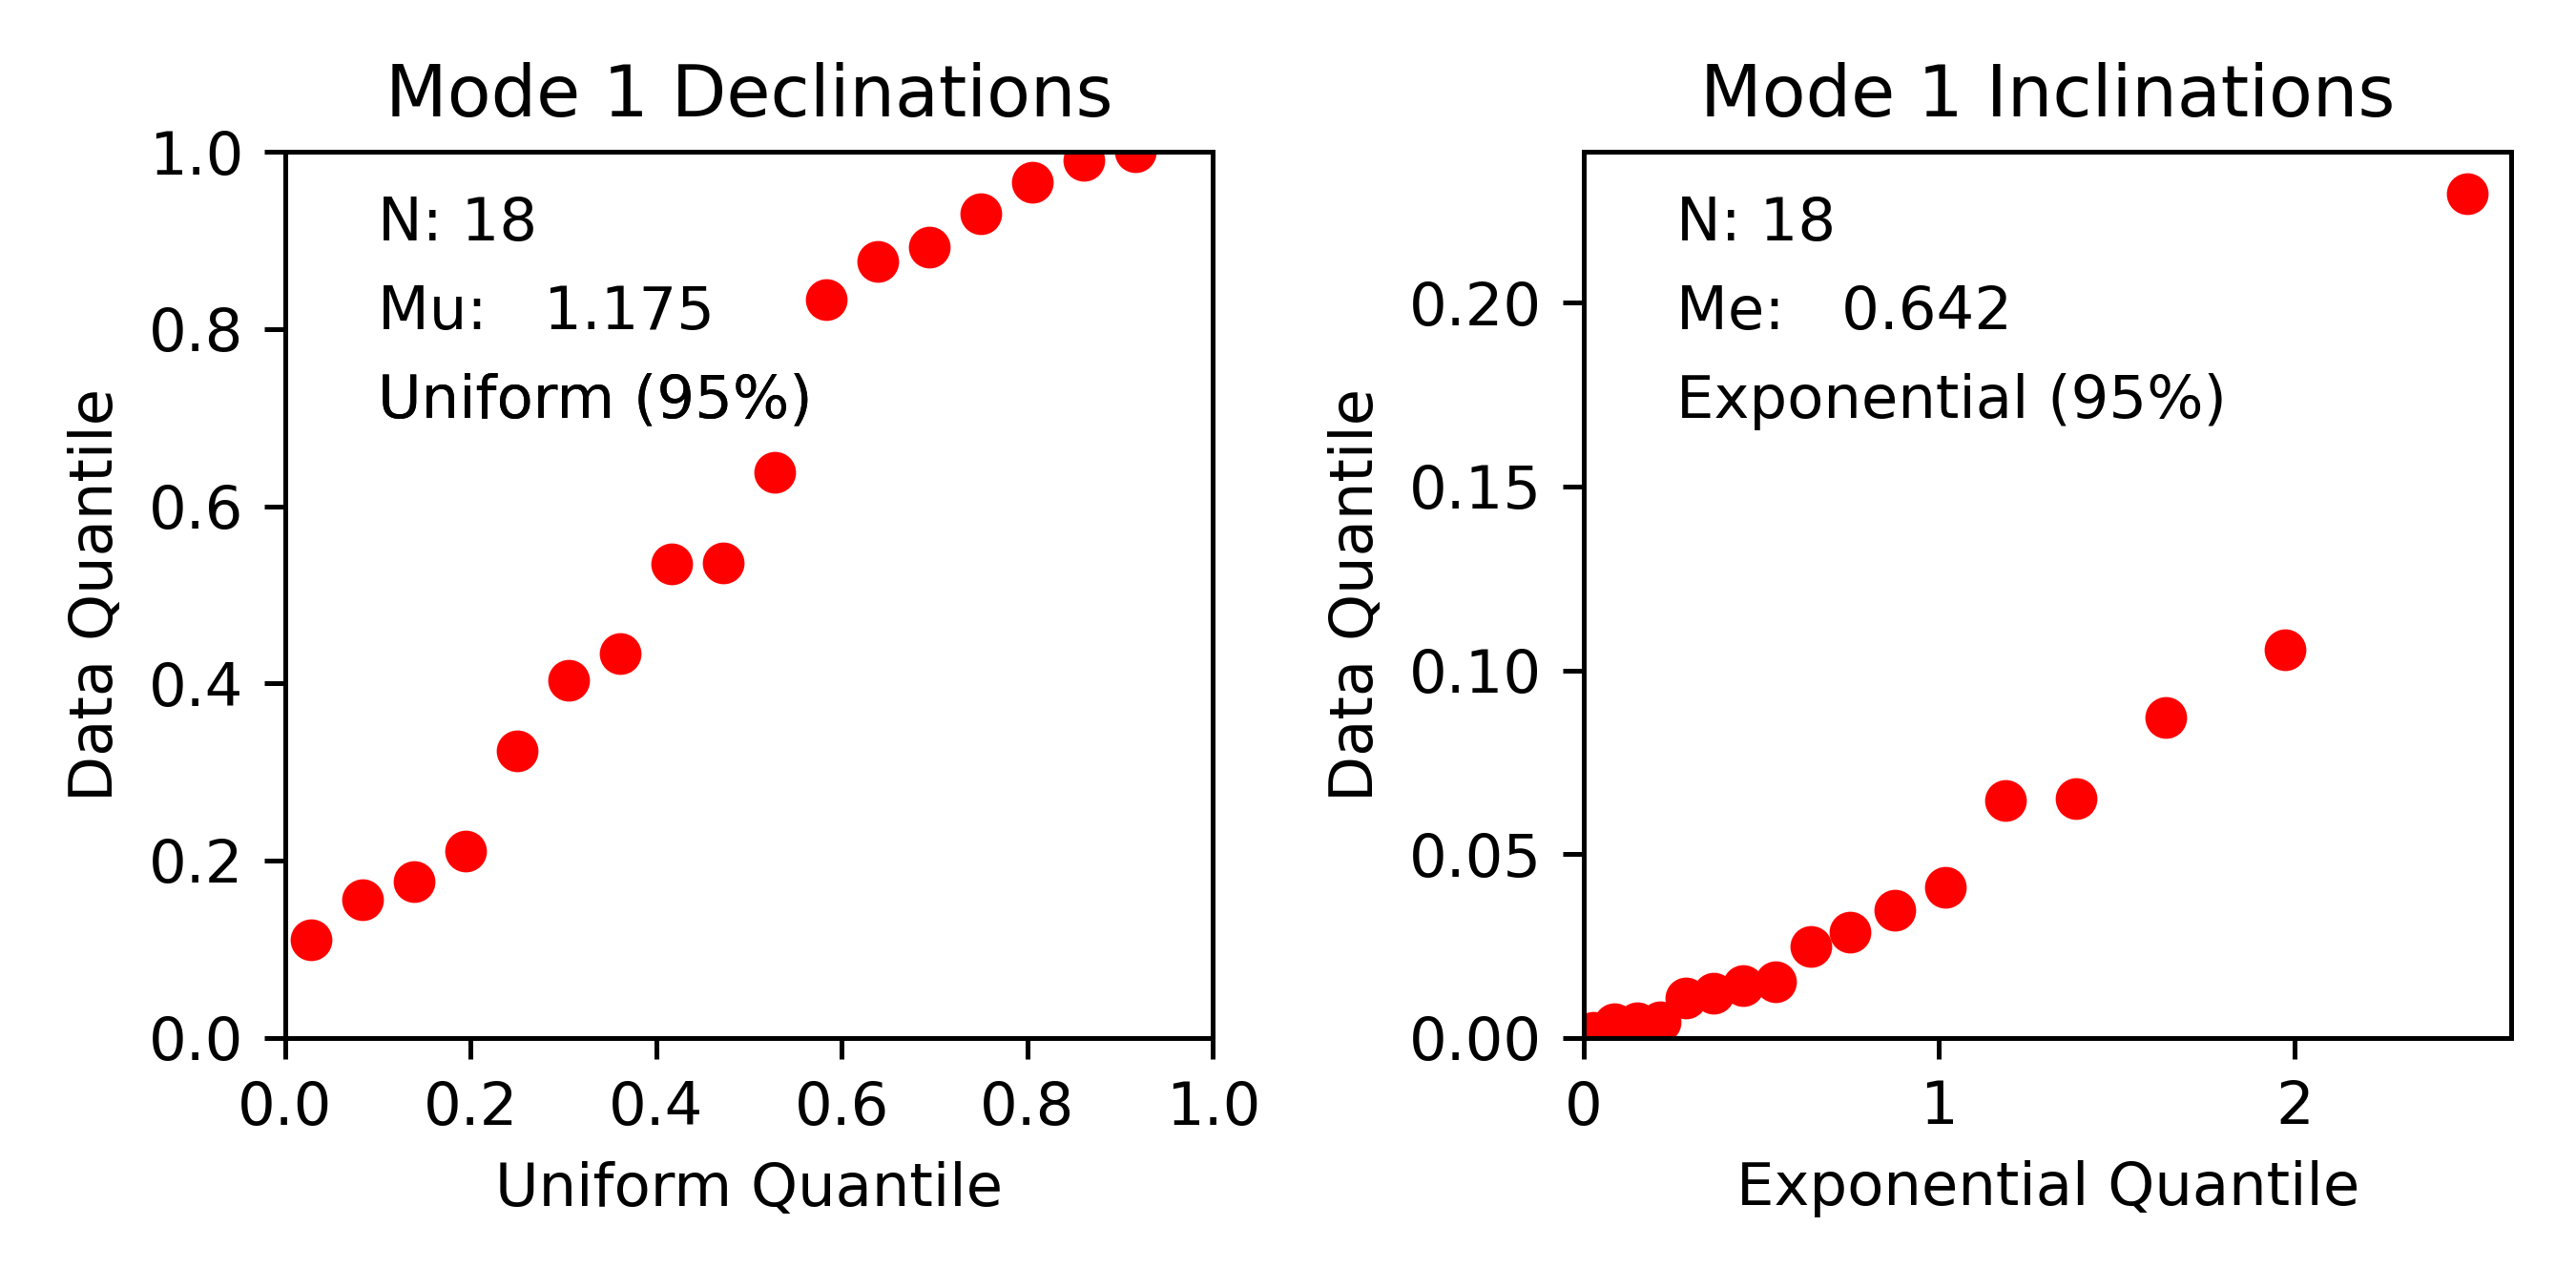
\includegraphics[width=5.8 in]{figure/Zhang2024b/SI_Cardenas_QQ.png}
\caption[Cardenas Basalt VGPs Fisher distribution test]{Fisher quantile-quantile \cite{Fisher1987a} test of the distribution of the site level virtual geomagnetic poles of the Cardenas Basalt lava flows. The results show that the null hypothesis that the VGPs are Fisher-distributed cannot be rejected.}
\label{fig:Cardenas_QQ}
\end{figure}

\begin{figure}
\centering
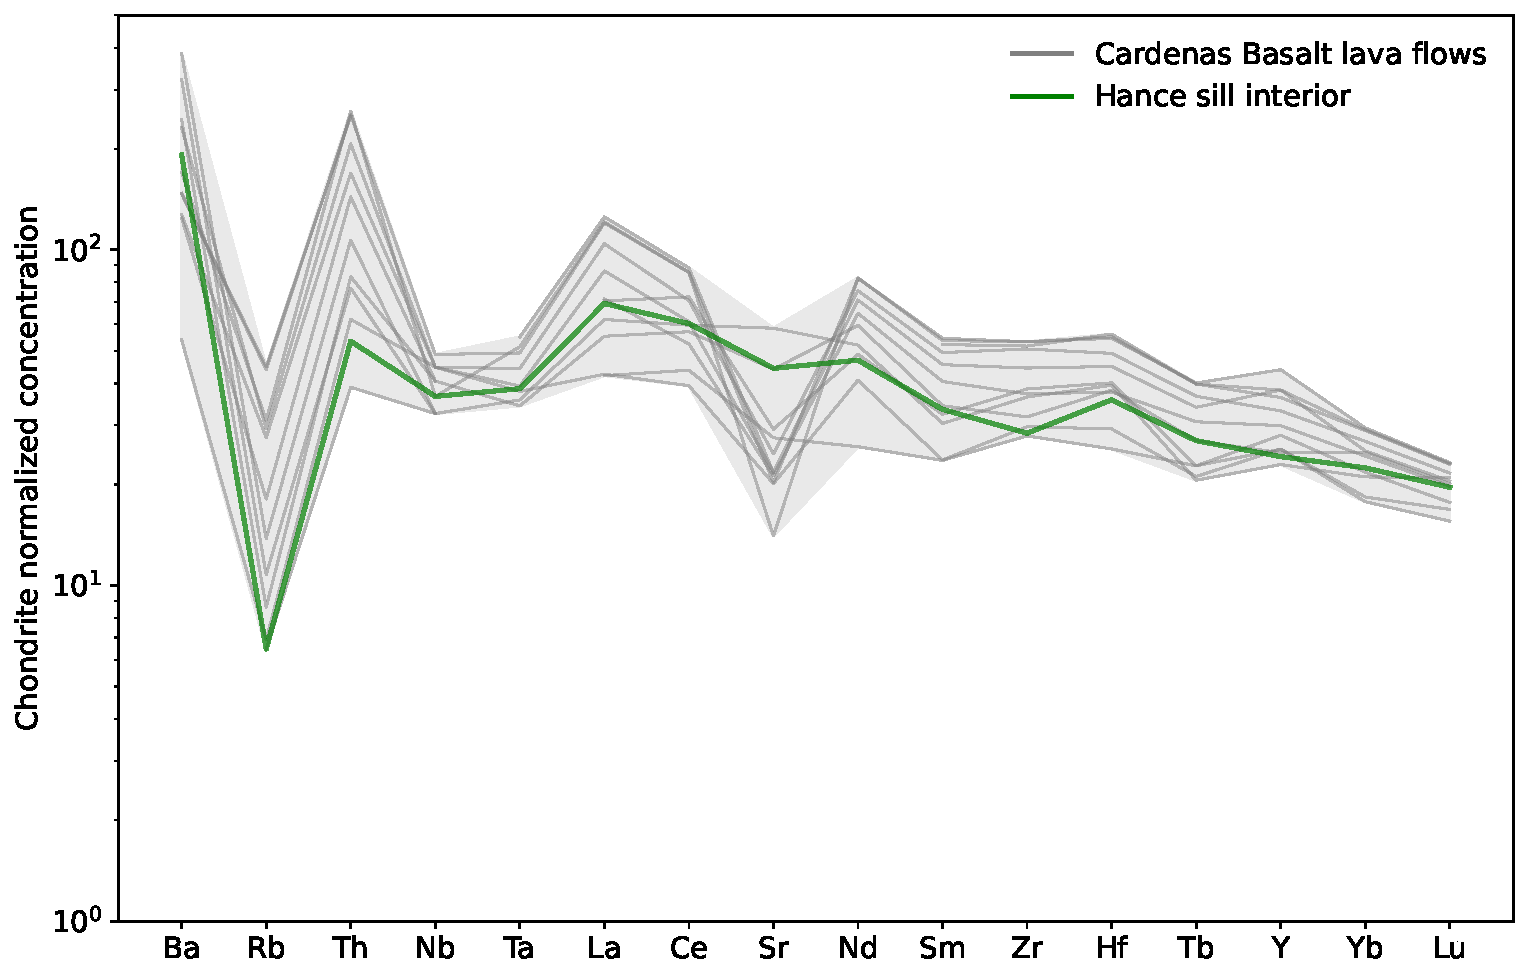
\includegraphics[width=0.7\textwidth]{figure/Zhang2024b/Larson1994a_trace_elements.pdf}
\caption[Trace element geochemistry data of the Cardenas Basalt and the Hance sill.]{Trace element geochemistry data from \cite{Larson1994a}. The elemental abundance of the interior of the Hance sill is similar to that of the Cardenas Basalt lavas. Virtual geomagnetic poles developed from the Hance sill, Hance dike, and another undated sill in Red Canyon adjacent to Hance rapids plot closer to those of the Cardenas Basalt than the dated ca. 1098 Ma poles as shown in the main text. These data are consistent with the interpretation that the intrusions near Hance rapids are feeders to the Cardenas Basalt.}
\label{fig:trace_elements}
\end{figure}


\begin{sidewaystable}
\tiny
\caption[Compilation of paleomagnetic data developed from mafic sills in central Arizona by \cite{Harlan1993a} and \cite{Donadini2011a}.]{\scriptsize Compilation of paleomagnetic data collected from mafic sills in central Arizona by \cite{Harlan1993a} and \cite{Donadini2011a}. The study of \cite{Donadini2011a} revisited some field areas of \cite{Harlan1993a} and resampled some diabase sills in the earlier study. However, the determination of individual cooling units was not clear in \cite{Donadini2011a}. We compiled data from both studies with a focus on distinguishing individual paleomagnetic sites as distinct cooling units based on geographic and paleomagnetic information provided in the original publications. Data rejected by the original authors are not included. Original ``site" level data with better Fisher statistics (higher concentration parameter k values) are preferentially used in cases where repeat sampling of the same cooling unit is interpreted to have happened. We interpret site GD12 and GD13 of \cite{Harlan1993a} are the same as site OD in \cite{Donadini2011a} and thus recalculated mean statistics. dir\_dec---declination; dir\_inc--- inclination; k---kappa concentration parameter of the site mean direction; a$_{95}$---95\% confidence angle of site mean direction; n---number of samples included in each site; N---number of sites used in calculating the mean statistics by polarity; plat/Plat---pole latitude; plon/Plon---pole longitude. The site level pole locations are recalculating using the directions and site location information provided in the original studies.}
\begin{tabular}{p{3cm}p{1cm}p{1cm}p{1cm}p{1cm}p{1cm}p{1.2cm}p{1cm}p{3cm}p{1cm}p{1cm}p{1cm}}

site                   & dir\_dec & dir\_inc & k     & a95  & n  & slon    & slat  & pole reference                      & plon  & plat  & polarity \\
\hline 
GD01-02                & 279.2    & 57       &       &      &    & 249.5   & 33.7  & Harlan, 1993                        & 188.7 & 26.4  & N        \\
GD03                   & 285.3    & 51.4     & 165   & 3.6  & 11 & 249.5   & 33.8  & Harlan, 1993                        & 180.7 & 28.8  & N        \\
GD04                   & 295.5    & 56.6     & 81.9  & 7.7  & 7  & 249.5   & 33.8  & Harlan, 1993                        & 182.9 & 38.4  & N        \\
GD05                   & 283.2    & 26       & 108.5 & 5.8  & 7  & 249.5   & 33.8  & Harlan, 1993                        & 163.9 & 18.4  & N        \\
GD06-07                & 282.8    & 48.9     &       &      &    & 249.3   & 33.5  & Harlan, 1993                        & 179.3 & 25.8  & N        \\
GD08                   & 318      & 61.2     & 56.1  & 5.6  & 13 & 249.3   & 33.5  & Harlan, 1993                        & 186.8 & 56.1  & N        \\
GD09                   & 299.2    & 53.8     & 21.1  & 11.5 & 9  & 249.3   & 33.5  & Harlan, 1993                        & 178.3 & 40.3  & N        \\
GD10                   & 267.5    & 38.2     & 421.5 & 3.3  & 6  & 249.3   & 33.5  & Harlan, 1993                        & 178.7 & 9.7   & N        \\
GD17                   & 285.9    & 17.1     & 34.5  & 8.3  & 10 & 249.1   & 33.6  & Harlan, 1993                        & 157.7 & 18    & N        \\
GD18-20                & 339.6    & 36.3     &       &      &    & 249.2   & 33.5  & Harlan, 1993                        & 128   & 67.5  & N        \\
GD22                   & 270.1    & 40.4     & 120.3 & 5.1  & 8  & 249.5   & 33.8  & Harlan, 1993                        & 178.9 & 12.7  & N        \\
GD24                   & 297.9    & 58.5     & 168   & 4    & 9  & 249.5   & 33.8  & Harlan, 1993                        & 184.8 & 40.8  & N        \\
GD29                   & 306.9    & 66.4     & 678.5 & 2    & 9  & 249.4   & 33.6  & Harlan, 1993                        & 197.2 & 48.2  & N        \\
GD30                   & 264.1    & 33.4     & 157.6 & 5.4  & 6  & 249.4   & 33.6  & Harlan, 1993                        & 177.8 & 5.3   & N        \\
DF                     & 332.6    & 69.4     & 145.1 & 3.5  & 13 & 249.3   & 33.5  & Donadini et al., 2011               & 212.7 & 62.5  & N        \\
DG                     & 266.2    & 34.4     & 58.7  & 8    & 7  & 249.4   & 33.6  & Donadini et al., 2011               & 176.9 & 7.4   & N        \\
DJ                     & 281.9    & 52.8     & 325.5 & 2.9  & 9  & -110.48 & 33.65 & Donadini et al., 2011               & 182.8 & 26.7  & N        \\
KD                     & 293.8    & 13.4     & 142.3 & 3.3  & 14 & -110.97 & 33.89 & Donadini et al., 2011               & 151.2 & 23.5  & N        \\
MD                     & 277.2    & 50.7     & 110.4 & 4.2  & 12 & -110.98 & 33.87 & Donadini et al., 2011               & 182.9 & 22.2  & N        \\
GD12\_GD13\_OD         & 280.8    & 45.7     & 313.7 & 7    &    & -110.98 & 33.81 & Harlan, 1993; Donadini et al., 2011 & 177.6 & 23    & N        \\
GD11                   & 115.3    & -69.9    & 173.7 & 4.2  & 8  & -110.96 & 33.75 & Harlan, 1993                        & 24.3  & -41   & R        \\
GD15-27                & 224.9    & -73.7    &       &      &    & -110.5  & 33.8  & Harlan, 1993                        & 103.8 & -50.9 & R        \\
BD                     & 137.6    & -74      & 66.1  & 8.2  & 7  & -110.61 & 33.61 & Donadini et al., 2011               & 36.5  & -52   & R        \\
WD                     & 199.2    & -71      & 92.1  & 3.1  & 24 & -110.69 & 33.55 & Donadini et al., 2011               & 95    & -64.4 & R        \\
                       &          &          &       &      &    &         &       &                                     &       &       &          \\
\hline 
                       & dir\_dec & dir\_inc & k     & a95  & N  & Plon    & Plat  & A95                                 &       &       &          \\
\hline 
normal polarity mean   & 287.6    & 47.4     & 14.4  & 8.5  & 20 & 177.4   & 30.6  & 8.9                                 &       &       &          \\
reversed polarity mean & 167.4    & -77      & 31.8  & 16.6 & 4  & 239.9   & 57.5  & 30.6                                &       &       &         
\end{tabular}

\end{sidewaystable}

\clearpage





